\documentclass[10pt]{article}

% Packages
\usepackage{graphicx}
\usepackage{subcaption}
\usepackage{fancyhdr}
\usepackage[margin=2cm]{geometry} % Set page margins
\usepackage{hyperref} % Required for adding hyperlinks
\usepackage{titlesec} % Customize section titles
\usepackage{lipsum} % For dummy text
\usepackage{enumitem} % For bullet point feature
\usepackage{float}
\usepackage{listings}
\usepackage{xcolor}
\lstset{
  language=Java,
  basicstyle=\ttfamily,
  keywordstyle=\color{blue}\ttfamily,
  stringstyle=\color{red}\ttfamily,
  commentstyle=\color{green}\ttfamily,
  morecomment=[l][\color{magenta}]{\#},
  showstringspaces=false,
  breaklines=true,
  tabsize=2
}

\pagestyle{fancy}
\fancyhf{}
\lhead{\includegraphics[width=1.5cm]{gw_pos_monogram.png}}
\rhead{CSCI 6461 Computer Systems and Architecture}
% Title page information
\title{%
  \textbf{\huge CSCI6461 Project Part III} \\
  \Large Project: Basic Machine Simulator
}
\author{
  Abhinava Phukan\\
  \texttt{abhinava.phukan@gwu.edu}
  \and
  Dev Shah\\
  \texttt{devshah7@gwu.edu}
  \and
  Natalie Rachel Jordan\\
  \texttt{nrj@gwu.edu}
  \and
  AlHassan Halawani\\
  \texttt{hassanhalawani@gwu.edu}
}
\date{\today}

% Section title formatting
\titleformat{\section}
{\normalfont\Large\bfseries}{\thesection}{1em}{}

% Begin document
\begin{document}

% Title page
\maketitle

% Abstract
\section*{Abstract}
To gain a deeper understanding of the design, structure and operations of a computer
system, principally focusing on the ISA and how it is executed. The Simulator built here
emulates small classical CISC computer which executes certain kind of instructions and how it handles
memory. This allows us to understand the Macro and micro structure of the CPU.

% Introduction
\section{Introduction}\label{section 1}
In order to run the jar file for Windows:\label{windowsetup}
\begin{itemize}[label=--]
  \item Ensure You have jdk-17 or above installed in your system.
  \item You have Java Development Kit Binaries location put as a reference for your command line arguments (System Environment Variables)
  \item Run The runsim.bat fil to start the Machine Simulator.
\end{itemize}
To run the jar file using a Mac system:\label{macsetup}
\begin{itemize}[label=--]
  \item Have jdk-17 or above installed in your system.
  \item Run the shell script provided to run the Machine Simulator
\end{itemize}
The use of a contrived CISC computer model facilitates understanding of the complex macro- 
and micro-structure of the CPU, including the components not visible to the programmer. 
Through simulating instruction execution, the model enables learners to better comprehend 
the underlying mechanisms of computer operation.
% Body
\section{Overview}
This section covers the structure of the program, its components \& features and 
a working demonstration of the example program.
\begin{figure}[H]
  \centering
  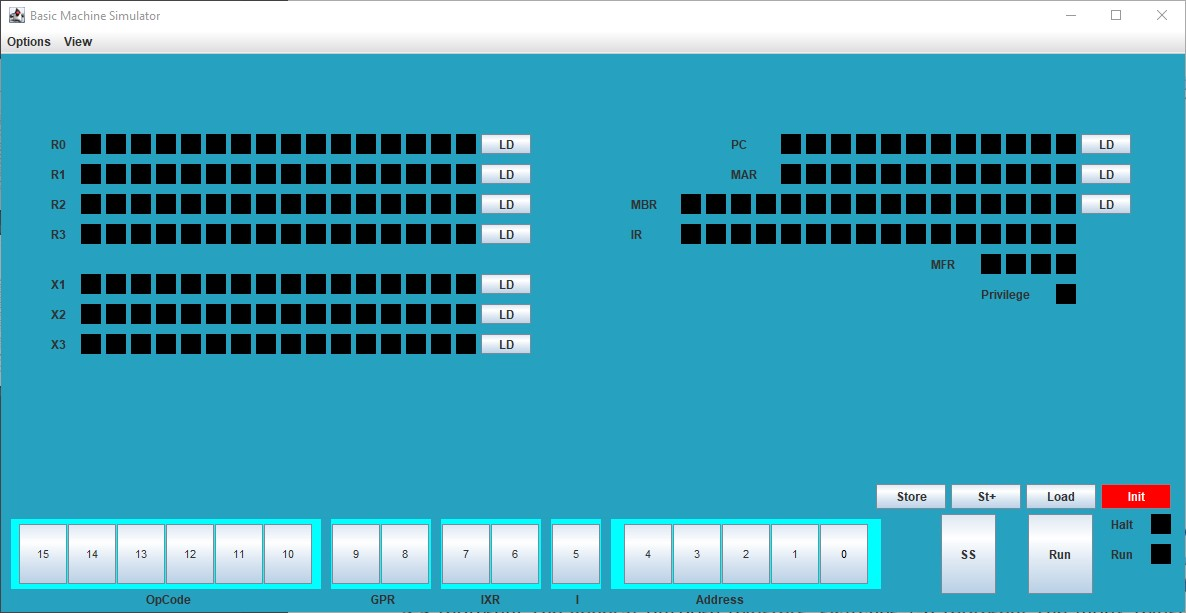
\includegraphics[width=1.0\textwidth]{Pics/Fig0.jpg}
  \caption{Gui Interface}
  \label{fig:gui_interface}
\end{figure}

\subsection{Understanding the Interface}
\subsubsection{Switches}
The computer simulator is designed to feature a 16-bit switch that enables the user to input binary 
values in a simple and intuitive manner. The switch is labeled from 0 to 15 in descending order, 
with each switch representing a specific bit in a binary number. The switch is segmented into separate 
sections that correspond to different components of a computer instruction. Switches 15-10 represent 
the opcode, switches 9-8 represent the general purpose registers, switches 7-6 represent the index register 
for addressing, and switch 5 represents the indirect bit for pointer addressing. Switches 4-0 represent the 
immediate address switch for accessing immediate addresses nearby.

\begin{figure}[H]
  \centering
  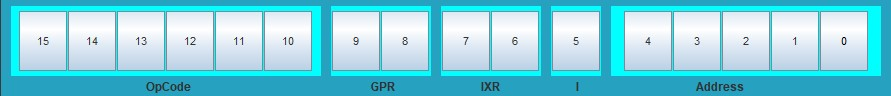
\includegraphics[width=1.0\textwidth]{Pics/Fig1.jpg}
  \caption{Switches}
  \label{fig:switches}
\end{figure}

By toggling these switches, the user can specify the instruction to execute, the registers to use, 
the index register to use for addressing, and whether to access data directly or indirectly. 
The 16-bit switch is a versatile and powerful tool for simulating computer instructions, and its 
user-friendly design facilitates ease of use.

\subsubsection{Load Button}
The computer simulator's graphical user interface (GUI) features Load buttons that are located adjacent to 
each register on the interface. These buttons allow the user to input data in the form of a 16-bit binary number
, which can be used for various purposes, such as specifying the value of a register or providing input for an 
instruction.

\begin{figure}[H]
  \centering
  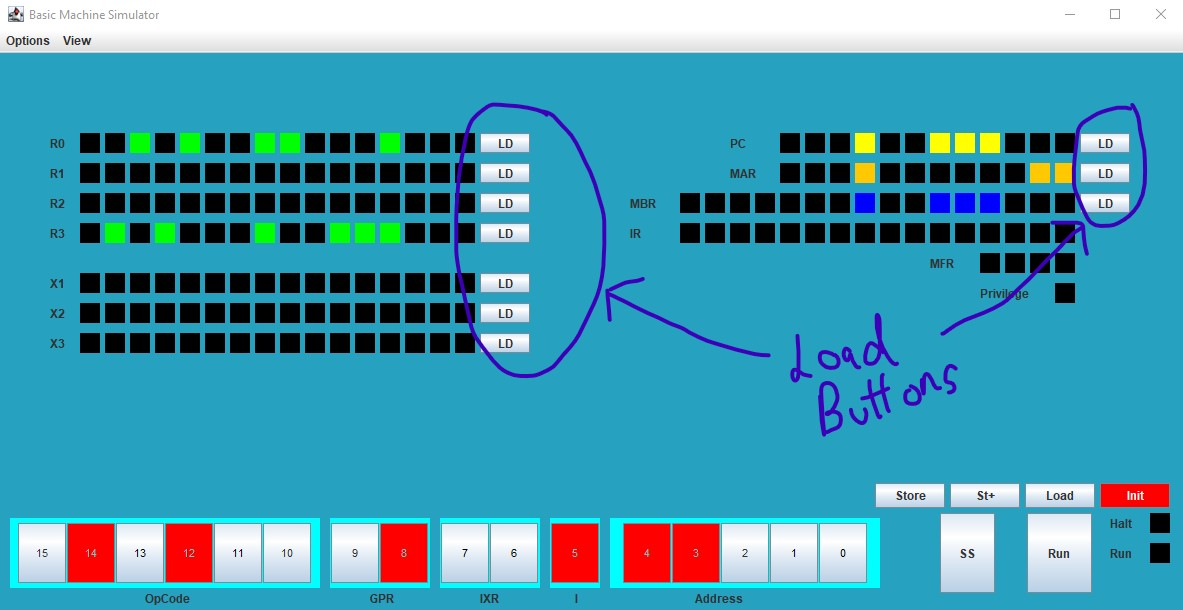
\includegraphics[width=0.75\textwidth]{Pics/Fig2.jpg}
  \caption{Load Buttons in Gui Simulator}
  \label{fig:ld_button}
\end{figure}
However, it should be noted that the Instruction Register (IR), Memory Fault Register (MFR), and Privilege (1 bit) 
registers do not have corresponding Load buttons. This is because the IR and MFR registers are used for internal 
functions of the simulator, while the Privilege bit is used to determine 
whether a user is in a privileged mode or not.

The binary number is input by toggling the switches provided, which represent the 0s and 1s in the binary number. 
Once the desired binary number is displayed on the switches, the user can click the LD button provided to 
load the binary number into the corresponding register. This makes it easy for the user to input data into the 
simulator and work with the registers efficiently.

\subsubsection{Control Buttons}
The simulator is designed to provide users with six buttons that allow them to interact with the program directly. 
These buttons are crucial in storing and loading data, initializing the system, and executing instructions. 
Here's a breakdown of each button's functionality:
\begin{figure}[H]
  \centering
  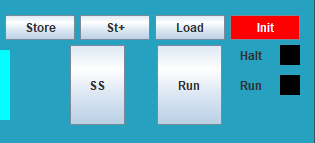
\includegraphics[width=0.5\textwidth]{Pics/Fig3.png}
  \caption{Control Buttons in Gui Simulator}
  \label{fig:ctrl_button}
\end{figure}
\begin{enumerate}
  \item Store Button: This button allows users to store data into the Data array of the system's memory. 
  When the user clicks on the Store button, the simulator reads the value in the Memory Address Register (MAR) 
  and the value in the Memory Buffer Register (MBR). It then uses the value stored in the MAR, 
  which is a 12-bit index value, to locate a specific memory location in the Data array. 
  Once the location is found, the 16-bit value in the MBR is stored in that location.\newline 
  i.e., Data[value(MAR)] = value(MBR).

  \item Store+ Button: This button works similarly to the Store button but with an additional feature. 
  After storing the data, the MAR is automatically incremented by 1, which allows users to continuously 
  store values in sequence.
  
  \item Load Button: This button allows users to load data from the Data array into the MBR. When the 
  Load button is clicked, the simulator reads the value in the MAR, uses it as an index value to locate a 
  specific memory location in the Data array, and loads the value stored in that location into the MBR.
  
  \item Init: This button opens a file dialog that prompts the user to provide the location of the program that needs 
  to be run on the simulator. Once the program is loaded, the instructions or other values are loaded into the 
  Data array based on the memory location specified in the file.
  \begin{figure}[H]
    \centering
    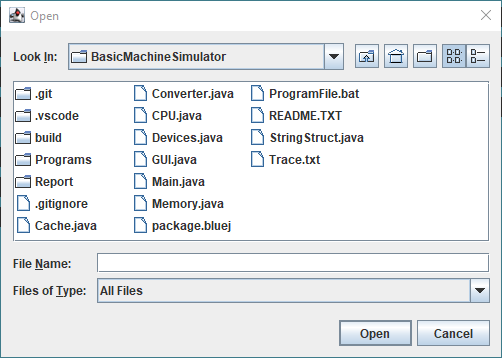
\includegraphics[width=0.5\textwidth]{Pics/Fig4.png}
    \caption{Init button on pressing gives file dialog}
    \label{fig:init_button}
  \end{figure}
  \item SS: The Single Step (SS) button takes a peek at the Program Counter (PC) Register, which stores the 
  address of the next instruction to be executed. It then loads the value in the PC into the Instruction 
  Register (IR) and executes the opcode, allowing the user to execute instructions one by one.
  
  \item Run: This button runs the program stored in the memory location specified by the PC. 
  Users can manually set the entry point of the program using the Load (LD) button. The program will continue 
  to run until it encounters a halt instruction that brings the system to a halt. These buttons provide 
  users with an intuitive way to interact with the simulator, allowing them to perform various tasks efficiently.
\end{enumerate}

\subsubsection{Menubar Buttons}
In addition to the buttons on the GUI interface, the menu bar in the simulator has additional features to 
enhance the simulation experience. The first feature, labeled as "Options", provides two options to the user. 
The first option is to reset the halted state of the machine, allowing the user to continue using the simulator. 
Once the machine is halted, the user cannot use the simulator unless the halt is reset. 
The second option in this menu is to reset the entire memory of the simulator, which zeros the data array 
and sets the register state and its bits to all zero, giving the user a fresh start.

The second feature in the menu bar, labeled as "View," provides the user with additional options to view the 
console monitor, console keyboard, and the cache. Additionally, users can attach virtual devices to the simulation 
to further enhance their experience. Overall, these features in the menu bar provide users with more control 
and flexibility in using the simulator, making it a powerful tool for learning and experimenting with computer 
architecture.

\subsection{Structure of the Program}
\begin{figure}[H]
\centering
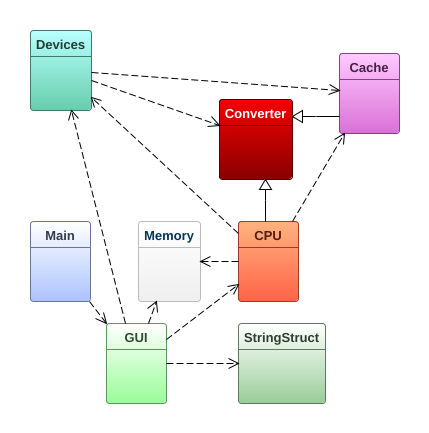
\includegraphics[width=0.5\textwidth]{Pics/class_diagram.png}
\caption{Class Diagram of the Simulator}
\label{fig:class_diagram}
\end{figure}
\begin{itemize}
  \item The program starts with the main class as the entry point, and upon running, it invokes the GUI from the GUI class. 
  The GUI class is responsible for creating the user interface and is highly dependent on other classes to perform the 
  simulation effectively.
  \item To run the simulation, the GUI class relies heavily on the CPU, Memory, and Devices classes. These classes are 
  responsible for executing the instructions of the simulated machine, storing and retrieving data, and interacting 
  with various devices that the machine may have.
  \item To run the simulation, the GUI class relies heavily on the CPU, Memory, and Devices classes. These classes are 
  responsible for executing the instructions of the simulated machine, storing and retrieving data, and interacting 
  with various devices that the machine may have.
  \item In addition to the core classes, the program also includes several helper classes to perform specific tasks. 
  The Converter class is used to convert binary numbers to decimal and vice versa. This conversion is a crucial 
  component of simulating a computer, as all data is represented in binary form.
  \item Similarly, the StringStruct class exists to facilitate custom string operations that may be required during 
  the simulation. This class may be used to format data or display messages to the user.
  \item Another essential component of the simulator is the Cache class, which is responsible for storing simple lines 
  of data in a first-in, first-out (FIFO) fashion. This caching mechanism helps speed up the simulation by reducing 
  the number of times the program needs to access data from memory.
  \item Lastly, it is worth noting that the Converter class is extended by both the CPU and Cache classes. 
  This extension ensures that all classes within the program can perform the necessary conversions with ease, 
  allowing for a seamless simulation experience.
\end{itemize}

\subsection{Running The Program}
Following will be the instructions to run on a packaged jar file:
\subsubsection{For Windows}\label{steps_for_windows}
\begin{enumerate}
  \item Extracting the zip file and open the directory.
  \item Ensure that you have java installed as per conditions provided on \hyperref[windowsetup]{Introduction}.
  \item Look for a batch file called runsim.bat. It will run the program.
  \item To run the program click on the init button that would bring the file dialogbox.
  \begin{figure}[H]
    \centering
    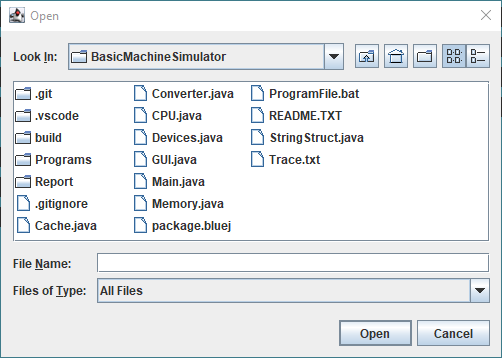
\includegraphics[width=0.5\textwidth]{Pics/Fig4.png}
    \caption{Activating File Dialog Box}
    \label{fig:fileDialog}
  \end{figure}
  \item Navigate the Program folder and choose which program you would like to run.
  \begin{figure}[H]
    \centering
    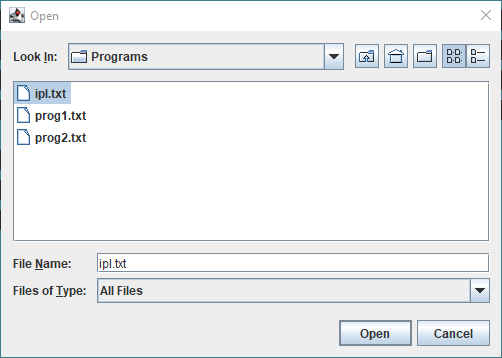
\includegraphics[width=0.5\textwidth]{Pics/Fig5.png}
    \caption{Choosing ipl.txt file as demo}
    \label{fig:Choosing File}
  \end{figure}
  \item On Accepting the file click ok then you will see in the console the lines of code that has been loaded into
  the memory.
  \begin{figure}[H]
    \centering
    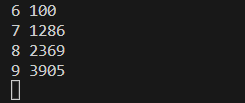
\includegraphics[width=0.5\textwidth]{Pics/Fig6.png}
    \caption{Loading Code}
    \label{fig:CodeLoading}
  \end{figure}
  \item Press those switch buttons to set the value where entry point of the program is located.
  \begin{figure}[H]
    \centering
    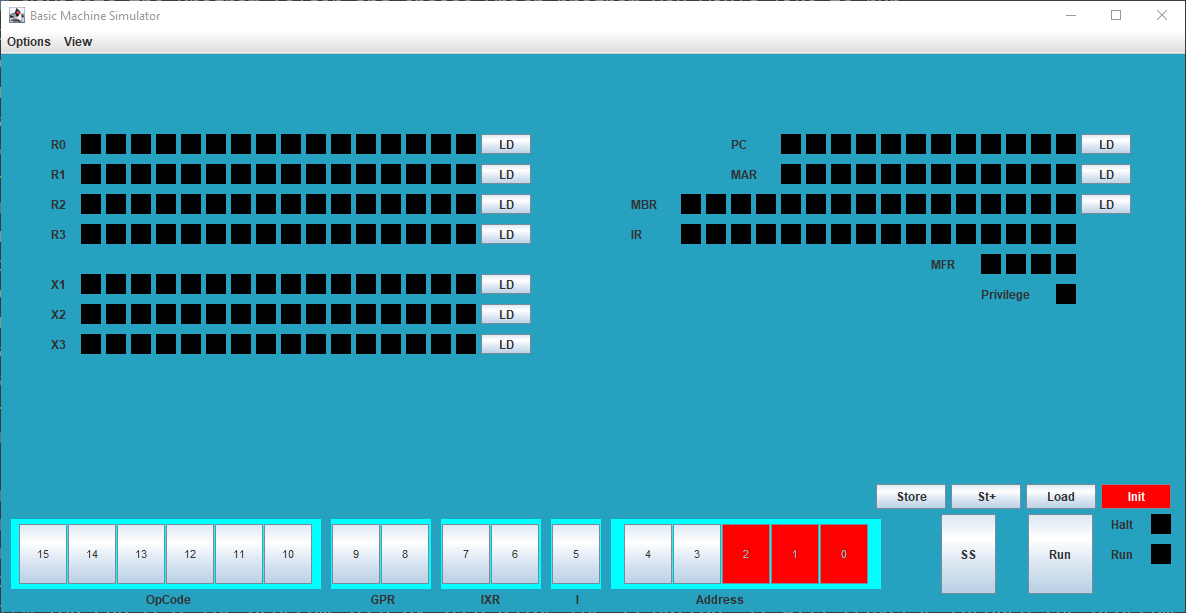
\includegraphics[width=0.5\textwidth]{Pics/Fig7.png}
    \caption{Pressing the switch}
    \label{fig:SwitchPress}
  \end{figure}
  \item Load the value in the switch to the Program Counter (PC) by pressing the LD button adjacent to it.
  \item Once the Value is loaded it would turn on the simulated LEDs.
  \begin{figure}[H]
    \centering
    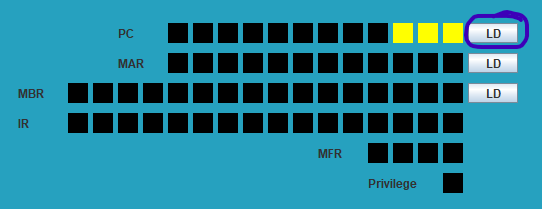
\includegraphics[width=0.5\textwidth]{Pics/Fig8.png}
    \caption{Load the entry point into PC}
    \label{fig:LoadPC}
  \end{figure}
  \item Here you have to options:
  \begin{itemize}
    \item You can test the program step by step using the SS button. It will traverse through the program
    normally as the Program Counter is incremented.
    \begin{figure}[H]
      \centering
      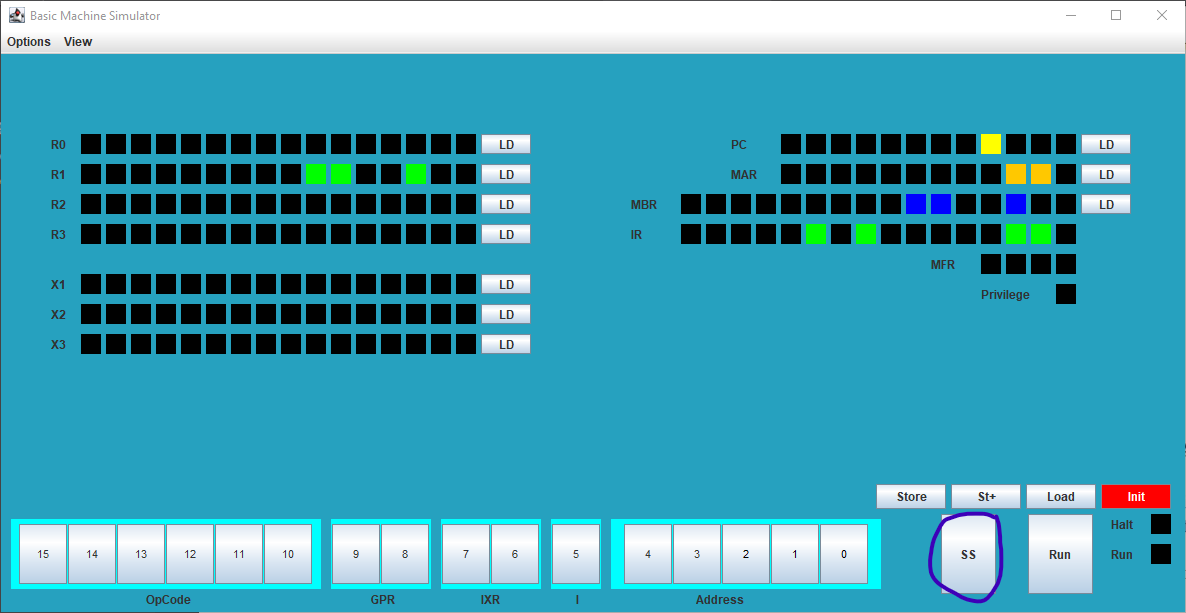
\includegraphics[width=0.5\textwidth]{Pics/Fig9.png}
      \caption{After Pressing the SS Button on ipl.txt}
      \label{fig:SSButton}
    \end{figure}
    \item You can run the program directly by using the run Button. As soon as the Run button is pressed, the
    PC will increment or jump to other instructions on its own and the Run indicator will turn GREEN.
    Once the program comes to a halt, the halt LED indicator will turn RED and the Run indicator will turn BLACK. 
    After this no more programs can be run unless it is reset in the options menu.
    \begin{figure}[H]
      \centering
      \begin{subfigure}[b]{0.48\textwidth}
        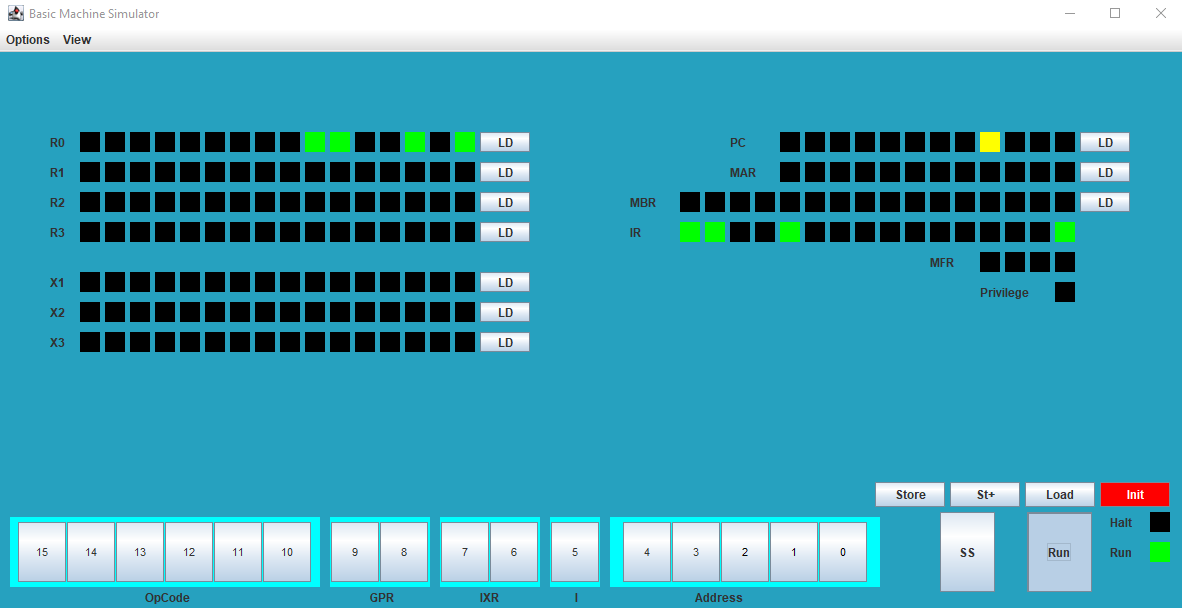
\includegraphics[width=\textwidth]{Pics/Fig10.png}
        \caption{Running the prog2.txt.}
        \label{fig:ProgramRun}
      \end{subfigure}
      \hfill
      \begin{subfigure}[b]{0.48\textwidth}
        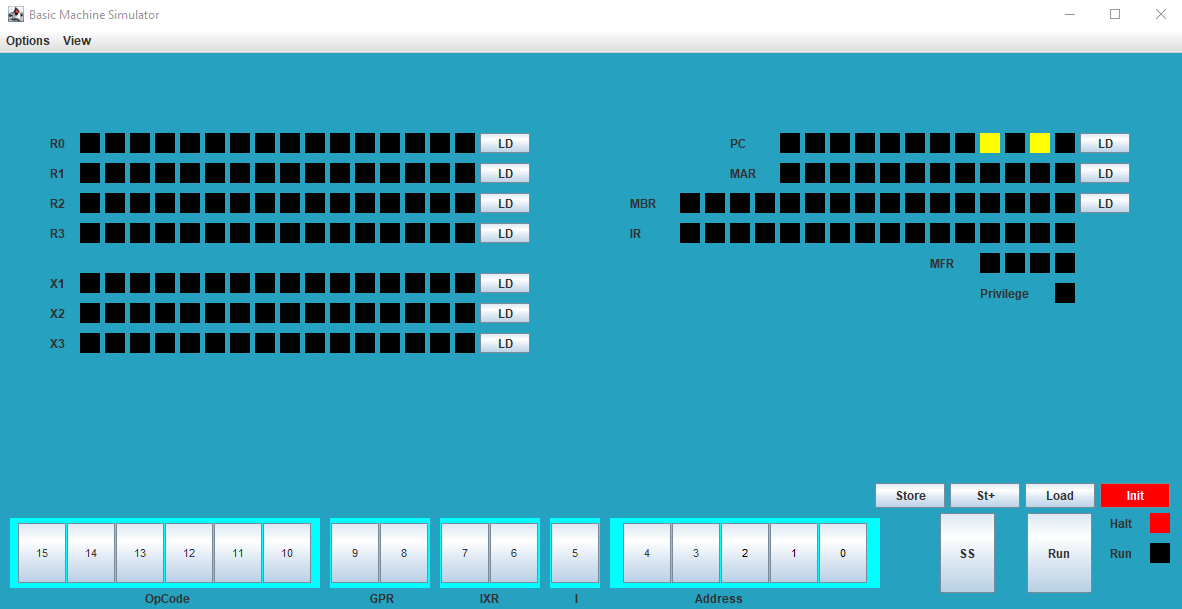
\includegraphics[width=\textwidth]{Pics/Fig11.png}
        \caption{Prog2.txt halting after completion.}
        \label{fig:ProgramHalt}
      \end{subfigure}
    \end{figure}
  \end{itemize}
\end{enumerate}
\subsubsection{For Mac Systems}
\begin{enumerate}
  \item Extract the zip file and open the extracted directory.
  \item Ensure your java is setup before continuing as per instructions 
  provided on \hyperref[macsetup]{Introduction}.
  \item Run the runsim.sh file to start the file.
  \item Follow the steps followed on the \hyperref[steps_for_windows]{Windows section} 
  when the program is activated and run.
\end{enumerate}
\subsection{Viewing the cache}
Since the Console printer and keyboard is attached alongside the cache, Go to view in the menu and 
view the cache and the console Option. The figure below shows the cache trace. More about the additional
features will be discussed in the next section.
\begin{figure}[H]
  \centering
  \begin{subfigure}[b]{0.48\textwidth}
    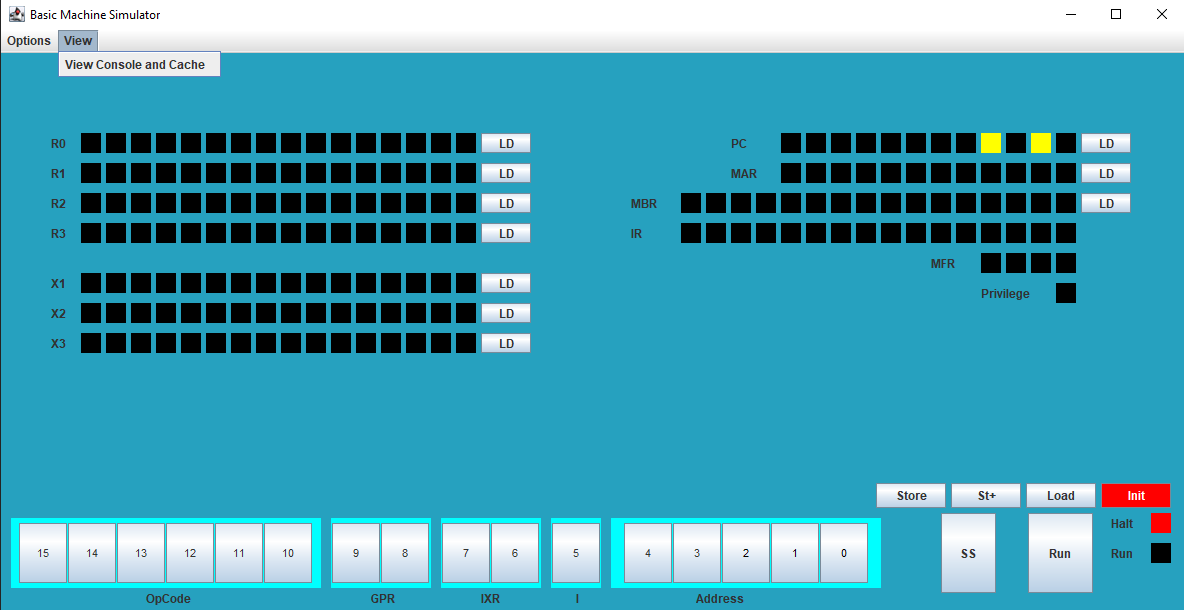
\includegraphics[width=\textwidth]{Pics/Fig12.png}
    \caption{Going to View Console and Cache.}
    \label{fig:ViewMenu}
  \end{subfigure}
  \hfill
  \begin{subfigure}[b]{0.48\textwidth}
    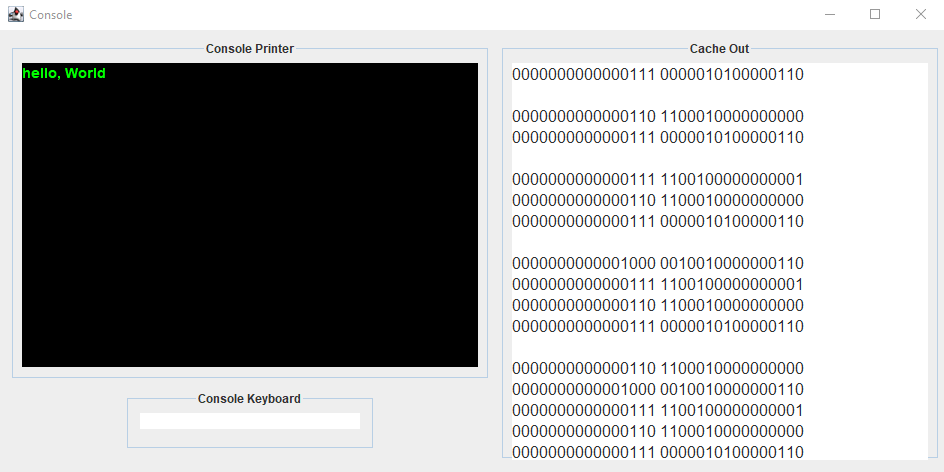
\includegraphics[width=\textwidth]{Pics/Fig13.png}
    \caption{Console and Cache.}
    \label{fig:ViewConsoleCache}
  \end{subfigure}
\end{figure}
% Feature Implementation
\section{Design Notes}
\subsection{CPU class structure}
\subsubsection{CPU Structure}
\begin{itemize}
  \item PC
  \item CC
  \item IR
  \item MAR
  \item MBR
  \item MFR
  \item R0,R1,R2,R3 (GPR)
  \item X1,X2,X3 (IXR)
  \item dev (for devices)
  \item cache (for cachelines)
\end{itemize}
\subsubsection{Instructions Implemented}
\begin{itemize}
  \item HLT (0x00), LDR (0x01), STR (0x02), LDA (0x03), LDX (0x21), STX (0x22).
  \item AMR (0x04), SMR (0x05), AIR (0x06), SIR (0x07).
  \item JZ  (0x08), JNE (0x09), JCC (0x0A), JMA (0x0B).
  \item JSR (0x0C), RFS (0x0D), SOB (0x0E), JGE (0x0F).
  \item MLT (0x10), DVD (0x11), TRR (0x12), AND (0x13), ORR (0x14), NOT (0x15).
  \item SRC (0x19), RRC (0x1A), IN  (0x31), OUT (0x32), CHK (0x33).
\end{itemize}

\subsection{Cache Implementation}
\begin{itemize}
  \item Cache is implemented by developing a Node structure for cache lines containing two
  members:
  \begin{itemize}[label=--]
    \item Key: Contains the address of the Program Counter
    \item Val: Contains the Value of the current IR.
  \end{itemize}
  \item Each Cache line is stored in form of an array following a FIFO structure.
\end{itemize}
The implementation of the structure is as follows:
\begin{lstlisting}[caption={Cache Struct Implementation Code}]
class CacheData{
    public short key;
    public short val;
}
public CacheData[] lines;
\end{lstlisting}
Here is the sample below for an output for cache:
\begin{figure}[H]
  \centering
  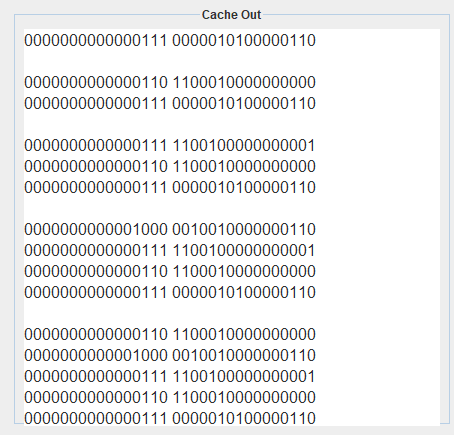
\includegraphics[width=0.65\textwidth]{Pics/Fig14.png}
  \caption{Sample Cache Output}
  \label{fig:Cache Output}
\end{figure}
\subsection{Devices Implementation}
The default main components added to the Simulator is the Console keyboard and the console printer:
\begin{figure}[H]
  \centering
  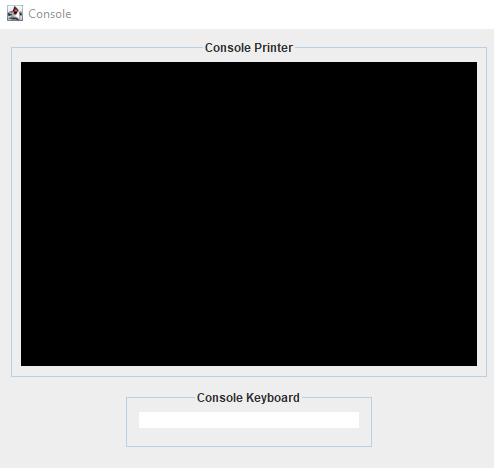
\includegraphics[width=0.4\textwidth]{Pics/Fig15.png}
  \caption{Console Printer and Console Keyboard}
  \label{fig:ConsolePrinterKeyboard}
\end{figure}
% References
\section{References}
List any sources you cited in your report.

\end{document}